% ********** Rozdział 4 **********
\chapter{Harmonogram realizacji projektu}
\section{Harmonogram realizacji projektu}
W tym rozdziale przedstawiono harmonogram projektu w formie diagramu Gantta. Jego celem jest graficzne zobrazowanie planu, etapów projektu oraz wzajemnych zależności czasowych między poszczególnymi zadaniami.

\subsection{Opis Diagramu Gantta}
Diagram Gantta prezentuje szczegółowy harmonogram realizacji projektu, w ramach którego wyróżniono następujące etapy:\\
\noindent\textbf{Tworzenie założeń projektu:} Przeprowadzenie analizy wymagań, sporządzenie dokumentacji oraz opracowanie planu realizacji.\\[1ex]
\noindent\textbf{Kodowanie:} Implementacja i integracja poszczególnych modułów aplikacji.\\[1ex]
\noindent\textbf{Tworzenie dokumentacji:} Opracowanie kompletnej dokumentacji technicznej oraz użytkowej.\\[1ex]
\noindent\textbf{Obrona projektu:} Przygotowanie prezentacji oraz obrona projektu przed komisją.


\begin{figure}[htbp]
  \centering
  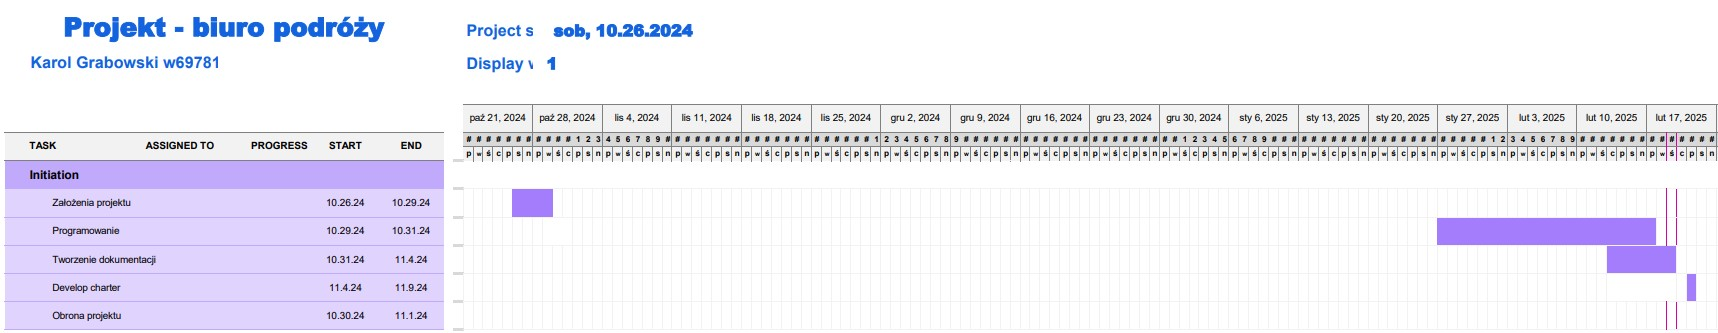
\includegraphics[width=1.1\textwidth]{figures/diagram_gannta.jpg} 
  \caption{Diagram Gantta przedstawiający harmonogram realizacji projektu}
  \label{fig:obrazek}
\end{figure}
\subsection{Napotkane problemy i trudności podczas realizacji projektu}
Podczas tworzenia systemu zarządzania biurem podróży napotkałem na kilka kluczowych wyzwań. Pierwszym z nich było ustalenie odpowiedniej architektury systemu. Zależało mi na tym, aby był on modułowy i skalowalny, co oznaczało łatwość w dodawaniu nowych funkcjonalności. W praktyce wymagało to oddzielenia modelu danych od logiki biznesowej oraz interfejsu użytkownika. Trudnością okazało się zaprojektowanie spójnego interfejsu komunikacyjnego między modułami, aby operacje związane z ofertami, rezerwacjami i płatnościami były zintegrowane i działały harmonijnie.

Kolejnym wyzwaniem było zarządzanie danymi. Przypisanie unikalnych identyfikatorów do ofert, rezerwacji, płatności i użytkowników stanowiło problem, zwłaszcza na początku projektu. Zastosowanie funkcji takich jak „Any()” czy „Max()” w LINQ ułatwiło generowanie tych identyfikatorów, ale wymagało to starannego dopracowania logiki, aby uniknąć konfliktów i duplikacji. Dodatkowo, wdrożenie zapisu i odczytu danych w formacie JSON wymagało precyzyjnego typowania, szczególnie w przypadku wartości pieniężnych, gdzie użycie typu „decimal” było kluczowe dla zachowania dokładności. Na początku napotykano trudności związane z doborem odpowiednich opcji serializacji, co mogło prowadzić do utraty precyzji danych.

Obsługa plików oraz mechanizmy backupu stanowiły kolejny obszar wyzwań. System musiał regularnie zapisywać dane do pliku JSON oraz tworzyć kopie zapasowe, aby chronić informacje przed utratą. Problemy pojawiały się przy implementacji mechanizmu backupu – kluczowe było uwzględnienie sytuacji, w których plik docelowy już istniał, lub gdy występowały trudności z dostępem do dysku. W miarę postępu projektu optymalizacja operacji na plikach może stać się istotnym wyzwaniem, zwłaszcza przy większej liczbie rekordów, co może prowadzić do wąskich gardeł podczas zapisu i odczytu. Potencjalne rozwiązania obejmują wdrożenie mechanizmów buforowania lub migrację do bardziej zaawansowanej bazy danych.

Nie mniej ważnym aspektem była walidacja danych oraz zapewnienie intuicyjnego interfejsu użytkownika. Konieczne stało się wdrożenie mechanizmów sprawdzania poprawności danych wprowadzanych przez użytkowników, na przykład weryfikacja formatu cen czy dostępności miejsc. Początkowo pojawiały się błędy związane z nieprawidłowymi danymi, co wymagało dodatkowych korekt. Mimo że interfejs został zaprojektowany jako konsolowy, musiał być przejrzysty i czytelny, co nie zawsze było łatwe do osiągnięcia na etapie projektowania.

\section{Informacje o repozytorium}

Zarządzanie projektem odbywało się za pomocą systemu kontroli wersji Git, co pozwoliło na precyzyjne monitorowanie postępów. Ponadto, projekt był hostowany na platformie GitHub, zapewniającej łatwy dostęp do repozytorium oraz narzędzi wspierających współpracę i integrację z innymi systemami. Repozytorium można znaleźć pod adresem:\\

\url{https://github.com/grabowskikarol/w69781_Programowanie_Obiektowe/tree/main/Projekt_w69781/Biuro_podrozy}


% ********** Koniec rozdziału **********